\chapter{Semantic Web application architecture}
\label{ch4}

So far, we have seen how RDF can represent data in a distributed way
across the Web. As such, it forms the basis for the Semantic Web, a web
of data in which Anyone can say Anything about Any topic. The focus of
this book is modeling on the Semantic Web: describing and defining
distributed data in such a way that the data can be brought back
together in a useful and meaningful way. In a book about only modeling,
one could say that there is no room for a discussion of system
architecture---the components of a computer system that can actually use
these models in useful applications. But this book is for the working
ontologist who builds models so that they can be used. But used for
what? These models are used to build some application that takes
advantage of information distributed over the Web. In short, to put the
Semantic Web to work, we need to describe, at least at a high level, the
structure of a Semantic Web application---in particular, the components
that comprise it, the kinds of inputs it gets (and from where), how it
takes advantage of RDF, and why this is different from other application
architectures.

Many of the components of a Semantic Web application are provided both
as supported products by companies specializing in Semantic Web
technology and as free software under a variety of licenses. New
software is being developed both by research groups as well as product
companies on an ongoing basis. We do not describe any particular tools
in this chapter\footnote{W3C has a wiki page listing some tools
  {https://www.w3.org/2001/sw/wiki/Tools}}, but rather we discuss the
types of components that make up a Semantic Web deployment and how they
fit together.

\begin{itemize}
\item
  \emph{\textbf{RDF Parser/Serializer:}} We have already seen a number
  of serializations of RDF. An RDF parser reads text in one (or more) of these formats and
  interprets it as triples in the RDF data model. An RDF serializer does the reverse; it takes a set of triples and
creates a file that expresses that content in one of the serialization
forms.
\item
  \emph{\textbf{RDF Store:}} We have seen how RDF distributes data in
  the form of triples. An RDF store (sometimes called a triple store) is
  a database that is tuned for storing and retrieving data in the form
  of triples. In addition to the familiar functions of any database, an
  RDF store has the additional ability to merge information from
  multiple data sources, as defined by the RDF standard.
\item
  \emph{\textbf{RDF Query Engine:}} Closely related to the RDF store is
  the RDF query engine. The query engine provides the capability to
  retrieve information from an RDF store according to structured
  queries.
\item
  \emph{\textbf{Application:}} An application has some work that it
  performs with the data it processes: analysis, user interaction,
  archiving, and so forth. These capabilities are accomplished using
  some programming language that accesses the RDF store via queries
  (processed with the RDF query engine).
\item
  \emph{\textbf{Reasoning Engine:}} A \emph{reasoner} or \emph{reasoning engine} is closely related to the RDF store or
  query engine and provides the capability to infer logical consequences
  from RDF data and schemata.
\end{itemize}

Most of these components have corresponding components in a familiar
relational data-backed application. The relational database itself
corresponds to the RDF store in that it stores the data. The database
includes a query language with a corresponding query engine for
accessing this data. In both cases, the application itself is written
using a general-purpose programming language that makes queries and
processes their results. The parser/serializer has no direct counterpart
in a relational data- backed system, at least as far as standards go.
There is no standard serialization of a relational database that will
allow it to be imported into a competing relational database system
without a change of semantics. (This is a key advantage of RDF stores
over traditional data stores.)

In the following sections, we examine each of these capabilities in
detail. Since new products in each of these categories are being
developed on an ongoing basis, we describe them generically and do not
refer to specific products.

\section{RDF PARSER/SERIALIZER}

How does an RDF-based system get started? Where do the triples come
from? There are a number of possible answers for this, but the simplest
one is to find them directly on the Web.

Google can find millions of files with the extension .rdf. Any of these
could be a source of data for an RDF application. But these files are
useless unless we have a program that can read them. That program is an
RDF parser. RDF parsers take as their input a file in some RDF format.
Most parsers support all the standard RDF formats outlined in Chapter~\ref{ch3}. 
An RDF parser takes such a file as input and converts it into an
internal representation of the triples that are expressed in that file.
At this point, the triples are stored in the triple store and are
available for all the operations of that store.

The triples at this point could also be serialized back out, either in
the same text form or in another text form. This is done using the
reverse operation of the parser: the serializer. It is possible to take
a ``round-trip'' with triples using a parser and serializer; if you
serialize a set of triples, then you parse the resulting string with a
corresponding parser (e.g., a Turtle parser for a Turtle serialization),
and the result is the same set of triples that the process began with.
Notice that this is not necessarily true if you start with a text file
that represents some triples. Even in a single format, there can be many
distinct files that represent the same set of triples. Thus, it is not,
in general, possible to read in an RDF file,
export it again, and be certain that the resulting file will be
identical (character by character) to the input file.

\subsection{Other data sources}

Parsers and serializers based on the standard representations of RDF are
useful for the systematic processing and archiving of data in RDF. While
there are considerable data available in these formats, even more data
are not already available in RDF. Fortunately, for many common data
formats (e.g., tabular data), it is quite easy to convert these formats
into RDF triples.

We already saw how tabular data can be mapped into triples in a natural
way. This approach can be applied to relational databases or
spreadsheets. Tools to perform a conversion based on this mapping,
though not strictly speaking parsers, play the same role as a parser in
a semantic solution: They connect the triple store with sources of
information in the form of triples. Most RDF systems include a table
input converter of some sort. Some tools specifically target relational
databases, including appropriate treatment of foreign key references,
whereas others work more directly with spreadsheet tables. Tools of this
sort are called converters, since they typically convert information
from some form into RDF and often into a standard form of RDF like
Turtle. This allows them to be used with any other RDF. Another rich
source of data for the Semantic Web can be found in existing web
pages---that is, in HTML pages. Such pages often include structured
information, like contact information, descriptions of events, product
descriptions, publications, and so on. This information can be combined
in novel ways on the Semantic Web once it is available in RDF.

A related approach to encoding information in web pages is a trend that
goes by the name of microformats. The idea of a microformat is that some
web page authors might be willing to embed structured information in
their web pages. To enable them to do this, a standard vocabulary
(usually embedded in HTML as special tag attributes that have no impact
on how a browser displays a page) is developed for commonly used items
on a web page. Some of the first microformats were for business cards
(including, in the controlled vocabulary, names, positions, companies,
and phone numbers) and events (including location, start time, and end
time). One limitation of microformats is the need to specify a
controlled vocabulary and provide a parser that can process that
vocabulary. Wouldn't it be better if, instead, someone (like the W3C)
would simply specify a single syntax for marking up HTML pages with RDF
data? Then there would be a single processing script for all
microformats.

The W3C has proposed just such a format called RDFa. The idea behind
RDFa is quite simple: Use the attribute tags in HTML to embed
information that can be parsed into RDF. Just like microformats, RDFa
has no effect on how a browser displays a page. A number of search
engines (Google and Yahoo!) and retailers (BestBuy, Overstock.com) have
begun to adopt RDFa to provide machine processable Semantic Web data.
Facebook has adopted a variant of RDFa as part of the Open Graph
Protocol---a network of information available in Facebook. A web site
called schema.org is even maintained by several big players of the Web
to explain how to embed these metadata in a page and some recommended
vocabularies to cover most frequent topics.

RDFa provides two advantages for sharing data on the Web. First, from
the point of view of data consumers, it is easier to harvest the RDF
data from pages that were marked up with structured data extraction in
mind, than from sources that were developed without this intention. But,
more important, from the point of view of the content author, it allows
them to express the intended meaning of a web page inside the web page
itself. This ensures that the RDF data in the document matches the
intended meaning of the document itself. This really is the spirit of
the word semantic in the Semantic

Web---that page authors be given the capability of expressing what they
mean in a web page for a machine to read and use.

\section{RDF STORE}

A database is a program that stores data, making them available for
future use. An RDF data storage solution is no different; the RDF data
are kept in a system called an RDF store. It is typical for an RDF data
store to be accompanied by a parser and a serializer to populate the
store and publish information from the store, respectively. Just as is
the case for conventional (e.g., relational) data stores, an RDF store
may also include a query engine, as described in the next section.
Conventional data stores are differentiated based on a variety of
performance features, including the volume of data that can be stored,
the speed with which data can be accessed or updated, and the variety of
query languages supported by the query engine. These features are
equally relevant when applied to an RDF store.

In contrast to a relational data store, an RDF store includes as a
fundamental capability, the ability to merge two data sets together.
Because of the flexible nature of the RDF data model, the specification
of such a merge operation is clearly defined. Each data store represents
a set of RDF triples; a merger of two (or more) data sets is the single
data set that includes all and only the triples from the source data
sets. Any resources with the same URI (regardless of the originating
data source) are considered to be equivalent in the merged data set.
Thus, in addition to the usual means of evaluating a data store, an RDF
store can be evaluated on the efficiency of the merge process.

RDF store implementations range from custom programmed database
solutions to fully supported off-the-shelf products from specialty
vendors. Conceptually, the simplest relational implementation of a
triple store is as a single table with three columns, one each for the
subject, predicate, and object of the triple. Table~\ref{tab:ch3.14} shows some data
about Los Angeles Metro stations, organized in this way.

This representation should look familiar, as it is exactly the
representation we used to introduce
RDF triples in Chapter~\ref{ch3}. Since this fits in a relational database
representation, it can be accessed using conventional relational
database tools such as SQL. An experienced SQL programmer would have no
problem writing a query to answer a question like ``List the dc:title of
every instance of metro:Metro in the table.'' As an implementation
representation, it has a number of apparent problems, including the replication of information in the first column
and the difficulty of building indices around string values like URIs.

\begin{table}[h]
\centering
\begin{tabular}{||l l l ||} 
 \hline
 Subject&Predicate&Object \\ [0.5ex] 
 \hline\hline
metro:item0&rdf:type&metro:Metro \\
metro:item0&dc:title&``Allen Station'' \\
metro:item0&simile:address&``395 N. Allen Av., Pasadena 91106'' \\
metro:item1&rdf:type&metro:Metro \\
metro:item1&dc:title&``Chinatown Station'' \\
metro:item1&simile:address&``901 N. Spring St., Los Angeles 90012--1862'' \\
metro:item2&rdf:type&metro:Metro \\
metro:item2&dc:title&``Del Mar Station'' \\
metro:item2&simile:address&``230 S. Raymond Av., Pasadena 91105--2014'' \\
\hline
\end{tabular}
\caption{Names and Addresses of Los Angeles Metro Stations}
\label{tab:ch3.14}
\end{table}





It is not the purpose of this discussion to go into details of the
possible optimizations of the RDF store. These details are the topic of
the particular (sometimes proprietary) solutions provided by a vendor of
an off-the-shelf RDF store. In particular, the issue of building indices
that work on URIs can be solved with a number of well-understood data
organization algorithms. Serious providers of RDF stores differentiate
their offerings based on the scalability and efficiency of these
indexing solutions.

\subsection{RDF data standards and interoperability of RDF stores}

RDF stores bear considerable similarity to relational stores, especially
in terms of how the quality of a store is evaluated. A notable
distinction of RDF stores results from the standardization of the RDF
data model and RDF/XML serialization syntax. Several competing vendors
of relational data stores dominate the market today, and they have for
several decades. While each of these products is based on the same basic
idea of the relational algebra for data representation, it is a
difficult process to transfer a whole database from one system to
another. That is, there is no standard serialization language with which
one can completely describe a relational database in such a way that it
can be automatically imported into a competitor's system. Such a task is
possible, but it typically requires a database programmer to track down
the particulars of the source database to ensure that they are
represented faithfully in the target system.

The standardization effort for RDF makes the situation very different
when it comes to RDF stores. Just as for relational stores, there are
several competing vendors and projects. In stark contrast to the
situation for relational databases, the underlying RDF data model is
shared by all of these products, and, even more specifically, all of
them can import and export their data sets in any of the standard
formats (RDF/XML,Turtle, JSON-LD, N3, etc. ). This makes it a routine
task to transfer an RDF data set---or several RDF data sets---from one
RDF store to another. This feature, which is a result of an early and
aggressive standardization process, makes it much easier to begin with
one RDF store, secure in the knowledge that the system can be migrated
to another as the need arises. It also simplifies the issue of
federating data that are housed in multiple RDF stores, possibly coming
from different vendor sources.

\subsection{RDF query engines}

An RDF store is typically accessed using a query language. In this
sense, an RDF store is similar to a relational database or an XML store.
Not surprisingly, in the early days of RDF, a number of different query
languages were available, each supported by some RDF-based product or
open-source project. From the common features of these query languages,
the W3C has undertaken the process of standardizing an RDF query
language called SPARQL. We cover the details of the SPARQL query
language in Chapter~\ref{ch6}.

An RDF query engine is intimately tied to the RDF store. To solve a
query, the engine relies on the indices and internal representations of
the RDF store: the more finely tuned the store is to the query engine,
the better its performance. For large-scale applications, it is
preferable to have an RDF store and query engine that retain their
performance even in the face of very large data sets. For smaller
applications, other features (e.g., cost, ease of installation,
platform, open-source status, and built-in integration with other
enterprise systems) may dominate.

The SPARQL query language includes a protocol for communicating queries
and results so that a query engine can act as a web service. This
provides another source of data for the semantic web--- the so-called
\emph{SPARQL endpoints} provide access to large amounts of structured
RDF data. It is even possible to provide SPARQL access to databases that
are not triple stores, effectively translating SPARQL queries into the
query language of the underlying store. The W3C has recently begun the
process to standardize a translation from SPARQL to SQL for relational
stores.

\subsection{Comparison to relational queries}

In many ways, an RDF query engine is very similar to the query engine in
a relational data store: It provides a standard interface to the data
and defines a formalism by which data are viewed. A relational query
language is based on the relational algebra of joins and foreign key
references. RDF query languages look more like statements in predicate
calculus. Unification variables are used to express constraints between
the patterns.

A relational query describes a new data table that is formed by
combining two or more source tables. An RDF query can describe a new
graph that is formed by describing a subset of a source RDF graph. That
graph, in turn, may be the result of having merged together several
other graphs. The inherently recursive nature of graphs simplifies a
number of detailed issues that arise in table-based queries. For
instance, SPARQL has little need for a subquery construct; in many
cases, the same effect can be achieved with a single query. Similarly,
there is nothing corresponding to the special case of an SQL
``self-join'' in SPARQL.

In the special case in which an RDF store is implemented as a single
table in a relational database, any graph pattern match in such a
scenario will constitute a self-join on that table. Some end- developers
choose to work this way in a familiar SQL environment. Oracle takes
another approach to making RDF queries accessible to SQL programmers by
providing its own SPARQL extension to its version of SQL, optimized for
graph queries. Their SPARQL engine is smoothly integrated with the
table/join structure of their SQL scripting language.

\section{Application Code}

Database applications include more than just a database and query
engine; they also include some application code, in an application
environment, that performs some analysis on or displays some information
from the database. The only access the application has to the database
is through the query interface, as shown in Figure~\ref{fig:ch4.1}.

An RDF application has a similar architecture, but it includes the RDF
parser and serializer, converters, the RDF merge functionality, and the
RDF query engine. These capabilities interact with the application
itself and the RDF store as shown in Figure~\ref{fig:ch4.2}.

The application itself can take any of several forms. Most commonly, it
is written in a conventional programming language (Java, C, Python, and
Perl are popular options). In this case, the RDF capabilities are
provided as API bindings for that language. It is also common for an RDF
store to provide a scripting language as part of the query system, which
gives programmatic access to these capabilities in a way that is not
unlike how advanced dialects of SQL provide scripting capabilities for
relational database applications.

\begin{figure}
    \centering
    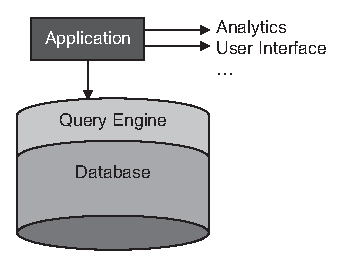
\includegraphics[width=5.0in]{media/ch4/f04-01-9780123859655.eps}
    \caption{Application architecture for a database application.}
    \label{fig:ch4.1}
\end{figure}


\begin{figure}
    \centering
    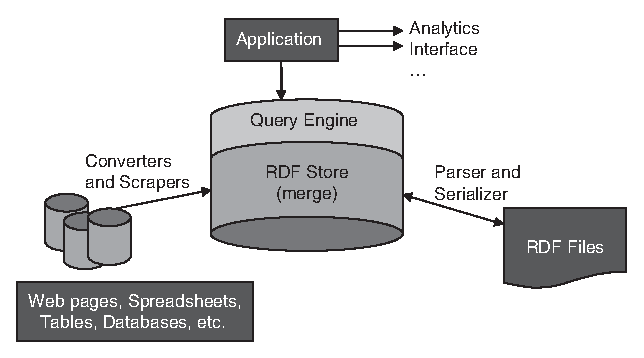
\includegraphics[width=5.0in]{media/ch4/f04-02-9780123859655.eps}
    \caption{Application architecture for an RDF application.}
    \label{fig:ch4.2}
\end{figure}

Regardless of the method by which the RDF store makes these
functionalities available to the application, it is still the
responsibility of the application to use them. Here are some examples of
typical RDF applications:

\begin{itemize}
    \item Calendar integration---shows appointments from different people and
teams on a single calendar view
    \item Map integration---shows locations of points of interest gathered from
different web sites, spreadsheets, and databases all on a single map
    \item Annotation---allows a community of users to apply keywords (with URIs)
to information (tagging) for others to consult
    \item Content management---makes a single index of information resources
(documents, web pages, databases, etc.) that are available in several
content stores.
\end{itemize}

The application will decide what information sources need to be scraped
or converted (e.g., diary entries in XML, lists of addresses from a web
page, directory listings of content servers).

Depending on the volatility of the data, some of this process may even
happen offline (e.g., locations of subway stations in New York, entries
in the Sears catalog, analyses of common chemical structures, etc.,
don't change very rapidly; these sorts of data could be imported into
RDF entirely outside of an application context), whereas other data
(like calendar data of team members, transactional sales data,
experimental results) will have to be updated on a regular basis. Some
data can remain in the RDF store itself (private information about this
team, order information, patented chemical formulas); other data could
be published in RDF form for other applications to use (train
timetables, catalog specials, FDA findings about certain chemicals).

Once all the required data sources have been converted, fetched, or
parsed, the application uses the merge functionality of the RDF store to
produce a single, federated graph of all the merged data. It is this
federated graph that the application will use for all further queries.
There is no need for the queries themselves to be aware of the
federation strategy or schedule; the federation has already taken place
when the RDF merge was performed.

From this point onward, the application behaves very like any other
database application. A web page to display the appointments of any
member of a team will include a query for that information. Even if the
appointments came from different sources and the information about team
membership from still another source, the query is made against the
federated information graph.

\subsection{RDF-backed web portals}

When the front end of an application is a web server, the architecture
(shown in Figure\ref{fig:ch4.1}) is well known for a database-backed web portal.
The pages are generated using any of a number of technologies (e.g.,
CGI, ASP, JSP, React, Angular) that allow web pages to be constructed
from the results of queries against a database. In the earliest days of
the web, web pages were typically stored statically as files in a file
system. The move to database-backed portals was made to allow web sites
to reflect the complex interrelated structure of data as it appears in a
relational database.

The system architecture outlined in Figure~\ref{fig:ch4.2} can be used the same way
to implement a Semantic Web portal. The RDF store plays the same role
that the database plays in database-backed portals. It is important to
note that because of the separation between the presentation layer in
both Figures \ref{fig:ch4.1} and \ref{fig:ch4.2}, it is possible to use all the same 
technologies for the actual web
page construction for a Semantic Web portal as those used in a
database-backed portal. But, in contrast to conventional data-backed web
portals, and because of the distributed nature of the RDF store that
backs a Semantic Web portal, information on a single RDF-backed web page
typically comes from multiple sources. The merge capability of an RDF
store supports this sort of information distribution as part of the
infrastructure of the web portal. When the portal is backed by RDF,
there is no difference between building a distributed web portal and one
in which all the information is local. Using RDF, federated web portals
are as easy as siloed portals.

\section{Data Federation}

The RDF data model was designed from the beginning with data federation
in mind. Information from any source is converted into a set of triples
so that data federation of any kind---spreadsheets and XML, database
tables and web pages---is accomplished with a single mechanism. As shown
in Figure~\ref{fig:ch4.2},

this strategy of federation converts information from multiple sources
into a single format and then combines all the information into a single
store. This is in contrast to a federation strategy in which the
application queries each source using a method corresponding to that
format. RDF does not refer to a file format or a particular language for
encoding data but rather to the data model of representing information
in triples. It is this feature of RDF that allows data to be federated
in this way. The mechanism for merging this information, and the details
of the RDF data model, can be encapsulated into a piece of
software---the RDF store---to be used as a building block for
applications.

The strategy of federating information first and then querying the
federated information store separates the concerns of data federation
from the operational concerns of the application. Queries written in the
application need not know where a particular triple came from. This
allows a single query to seamlessly operate over multiple data sources
without elaborate planning on the part of the query author. This also
means that changes to the application to federate further data sources
will not impact the queries in the application itself.

This feature of RDF applications forms the key to much of the discussion
that follows. In our discussion of RDFS and OWL, we will assume that any
federation necessary for the application has already taken place; that
is, all queries and inferences will take place on the federated graph.
The federated graph is simply the graph that includes information from
all the federated data sources over which application queries will be
run.

\section{Summary}

The components described in this chapter---RDF parsers, serializers,
stores, and query engines---are not semantic models in themselves but
the components of a system that will include semantic models. Even the
information represented in RDF is not necessarily a semantic model.
These are the building blocks that go into making and using a semantic
model. The model will be represented in RDF, to be sure. As we shall
see, the semantic modeling languages of the W3C, RDFS, and OWL are built
entirely in RDF, and they can be federated just like any other RDF data.

Where do semantic models fit into the application architecture of Figure~\ref{fig:ch4.2}? 
As data expressed in
RDF, they will be housed in the RDF store, along with all other data.
But semantic models go beyond just including data that will be used to
answer a query, like the list of plays that Shakespeare wrote or the
places where paper machines are kept. Semantic models also include
meta-data; data that help to organize other data. When we federate
information from multiple sources, the RDF data model allows us to
represent all the data in a single, uniform way. But it does nothing to
resolve any conflicts of meaning between the sources. Do two states have
the same definitions of ``marriage''? Is the notion of ``writing'' a
play the same as the notion of ``writing'' a song? It is the semantic
models that give answers to questions like these. A semantic model acts
as a sort of glue between disparate, federated data sources so we can
describe how they fit together.

Just as Anyone can say Anything about Any topic, so also can anyone say
anything about a model; that is, anyone can contribute to the definition
and mapping between information sources. In this way, not only can a
federated, RDF-based, semantic application get its information from
multiple sources, but it can even get the instructions on how to combine
information from multiple sources. In this way, the Semantic Web really
is a web of meaning, with multiple sources describing what the
information on the Web means.

\subsection{Fundamental concepts}

The following fundamental concepts were introduced in this chapter:

\emph{\textbf{RDF parser/serializer}}---A system component for reading and writing RDF
in one of several file formats.

\emph{\textbf{RDF store}}---A database that works in RDF. One of its main operations is
to merge RDF graphs. RDF query engine---This provides access to an RDF
store, much as an SQL engine provides access to a relational store.

\emph{\textbf{SPARQL}}---The W3C standard query language for RDF.

\emph{\textbf{SPARQL endpoint}}---An application that can answer a SPARQL query,
including one where the native encoding of information is not in RDF.

\emph{\textbf{Application interface}}---The part of the application that uses the
content of an RDF store in an interaction with some user.

\emph{\textbf{Converter}}---A tool that converts data from some form (e.g., tables) into
RDF.

\emph{\textbf{RDFa}}---Standard for encoding and retrieving RDF metadata from HTML
pages.
